\documentclass[aspectratio=169,usenames,dvipsnames]{beamer}


\usetheme{default}  % You can choose any other theme you prefer

\title{10 - Algoritmos}
\subtitle{Caminho Mínimo}
\author{Mateus Oliveira de Figueiredo}
\date{27/11/2023}

\usepackage{tikz}
\usetikzlibrary{matrix}
\usepackage{multicol}
\usepackage{algorithm}
\usepackage{algpseudocode}
\usepackage{xcolor}
\usepackage[utf8]{inputenc}
\usepackage[portuguese]{babel}
\usepackage{amsmath} % for "pmatrix" environment  
\usepackage{pgffor} 
\usepackage{listings}

\usepackage{pgfplots}
\DeclareUnicodeCharacter{2212}{−}
\usepgfplotslibrary{groupplots,dateplot}
\usetikzlibrary{patterns,shapes.arrows, positioning, arrows}
\usetikzlibrary{graphs, graphs.standard}
\pgfplotsset{compat=newest}

\lstset{
  language=Python,
  basicstyle=\ttfamily\tiny,
  keywordstyle=\color{blue},
  commentstyle=\color{green},
  stringstyle=\color{red},
  stepnumber=1,
  numbersep=10pt,
  showspaces=false,
  showstringspaces=false,
  tabsize=2,
  breaklines=true,
  breakatwhitespace=true,
}

\begin{document}

\begin{frame}
\titlepage
\end{frame}

\begin{frame}
\frametitle{Caminho Mínimo}

Dado um nó fonte encontrar o menor caminho para todos os outros nós.

\vfill
Algoritmos:
\begin{itemize}
  \item Dijkstra ($O(mlog(m))$)
  \item Bellman-Ford ($O(mn)$)
  \item Bellman-Ford com filas ($O(mn)$)
  \item DAGS ($O(m+n)$)
\end{itemize}
\vfill
\end{frame}


\begin{frame}
\frametitle{Proposição Relaxamento}

\vfill
\begin{block}{Proposição}
Seja G um dígrafo com fonte $s \in V$. Seja dist\_para um vetor de distâncias de s para cada vértice de G. 
Este vetor contém as distâncias mínimas se e somente se:
\begin{itemize}
  \item Para cada aresta $u \rightarrow v$ de G, temos que dist\_para[v] $\leq$ dist\_para[u] + peso(u,v).
  \item dist\_para[s] = 0
\end{itemize}
\end{block}
\vfill

\end{frame}

\begin{frame}{Bellman-Ford}
    Relaxar todas as arestas $|V|$ vezes.

    \vfill

    \onslide<2->{
        \begin{figure}[ht]
        \centering
        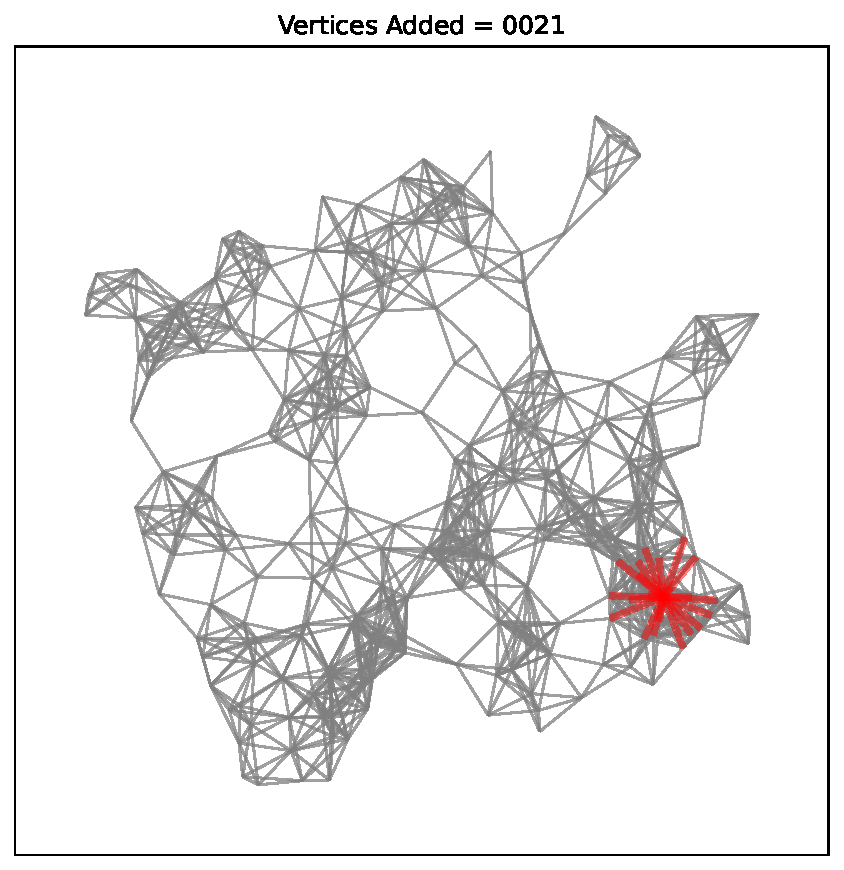
\includegraphics[width=0.4\textwidth]{figs/bellman/mediumEWD_0021.pdf}
        \end{figure}
    }

    \vfill
    \onslide<3>{
        \begin{itemize}
            \item Utilizar fila para guardar nós que devem ser relaxados
        \end{itemize}
    }

    \vfill

\end{frame}

\begin{frame}{Dijkstra} 

    A cada passo, relaxar o vértice com atual menor distância ao vértice fonte

    \vfill

    \onslide<2->{
        \begin{figure}[ht]
        \centering
        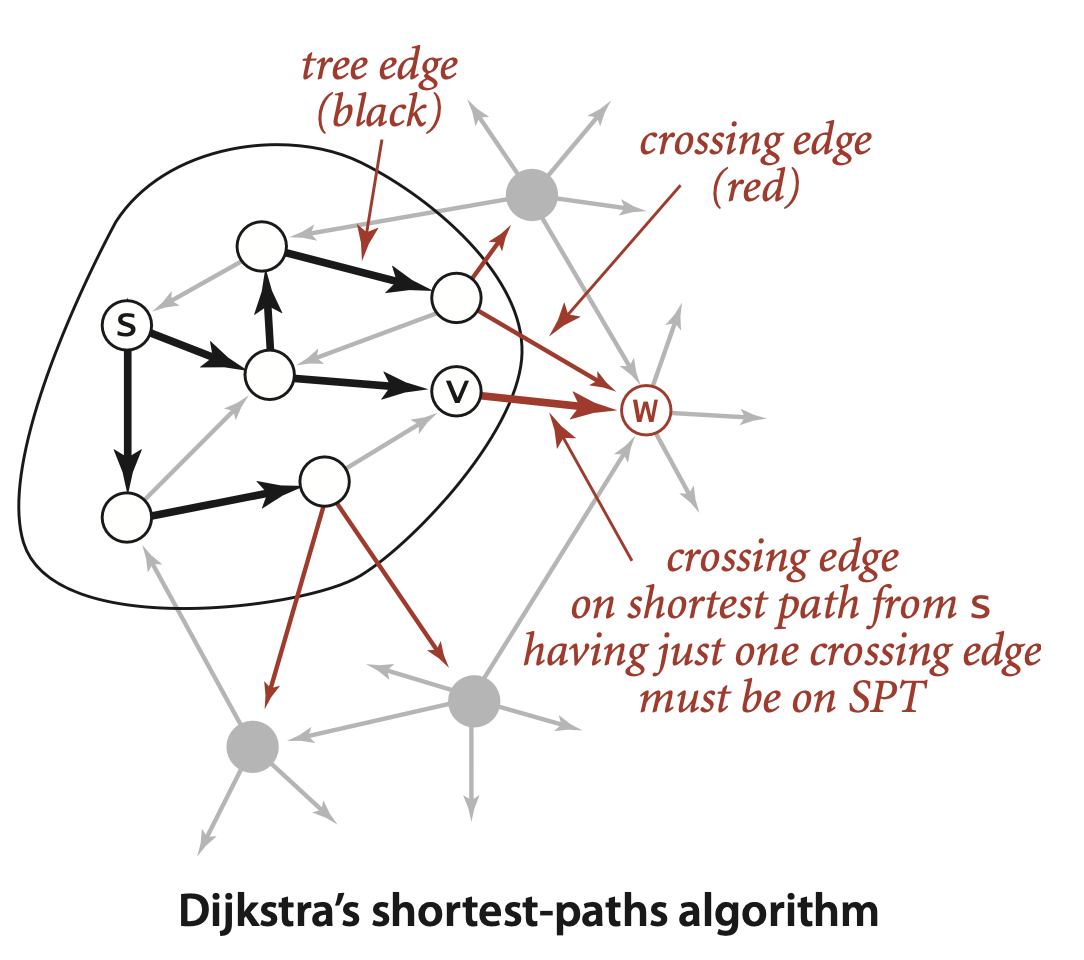
\includegraphics[width=0.4\textwidth]{figs/sedrick_dijkstra.png}
        %Add tiny caption with fig source
        \footnote{Algorithms Fourth Edition: Sedgewick, Wayne}
        \end{figure}
    }

    \vfill
    
\end{frame}

\begin{frame}{Dijkstra - IndexMinPQ}
    \vfill
    \begin{itemize}
        \item Heap que possui operações de alterar prioridade e remover o menor elemento em $O(log(n))$.
        \item Necessário quando aparece um caminho menor que o anterior. 
    \end{itemize}
    \vfill
\end{frame}


\begin{frame}{Resultados - Grafo Completo}
    \begin{columns}
    \column{0.5\textwidth}
        \begin{itemize}
            \item m = n(n-1)
            \item Pesos aleatórios no intervalo [0, 1]
        \end{itemize}
    \column{0.5\textwidth}
    \begin{figure}[ht]
        \centering
        \includegraphics<1>[width=0.9\textwidth]{figs/complete_graphs.pdf}
        \includegraphics<2>[width=0.9\textwidth]{figs/complete_graphs_log.pdf}
    \end{figure}

    \end{columns}

\end{frame}


\begin{frame}{Resultados - DAG Completo}
    \begin{columns}
    \column{0.5\textwidth}
        \begin{itemize}
            \item m = n(n-1)/2
            \item Pesos aleatórios no intervalo [0, 1]
        \end{itemize}
    \column{0.5\textwidth}
    \begin{figure}[ht]
        \centering
        \includegraphics<1>[width=0.9\textwidth]{figs/dag_graphs_0.pdf}
        \includegraphics<2>[width=0.9\textwidth]{figs/dag_graphs_1.pdf}
        \includegraphics<3>[width=0.9\textwidth]{figs/dag_graphs_log.pdf}
    \end{figure}

    \end{columns}

\end{frame}

\end{document}
